In this chapter we will briefly describe electronic voting in general, focusing mostly on the challenges and security parameters.

\section{Introduction}
In many aspects of our life's we in counter the act of voting, from simple things as voting whats for dinner, to the more complex things as a government election. The later involving a large number of people from different geographical locations. These election is normally handled by dividing the people into sections based on location, each section handling it's own sub-election and submitting the result to the overall tally.


\section{Classification}

\begin{description}
    
\item[DRE voting (Direct Recording Electronic)] is physically hardened electronic
equipment with special purpose voting software. The votes are
cast inside a voting booth at a polling site, however, cast votes are
recorded in electronic ballot boxes.

\item[Poll-site voting] does not use voting booths, but public computers at a
polling-site. The computers are connected over a closed and controlled
network.

\item[Poll-site kiosk voting] typically contains electronic voting terminals inside
a voting booth at a polling site (as in DRE voting). The terminals
are connected with a closed and controlled network.

\item[Poll-site Internet voting] provides a polling-site where users cast their
votes by using public computers. The computers at the site are online
over an uncontrolled network.

\item[Remote Internet voting] only requires Internet access and can be done
from your home computer. For authentication, the credentials of voters
are verified prior to the voting period through the use of a password
or some type of authentication token.

\end{description}


\section{The Voting Process}

There exists a wide variety of electronic voting systems and protocols, but
the main process is almost standard. The typical actors participating in any
voting system is described below [Cet09]:

\begin{description}
    \item[Voter] A voter is entitled to vote in the election, and has some private
        information that identifies it.

    \item[Registration authority] The registration authority ensures that only
        registered voters can vote (and only once).
        
    \item[Collection authority] The collection authority collects all cast votes.

    \item[Tallying authority] The tallying authority computes the result of the
        election and publishes it.   
\end{description}



\begin{figure}[H]
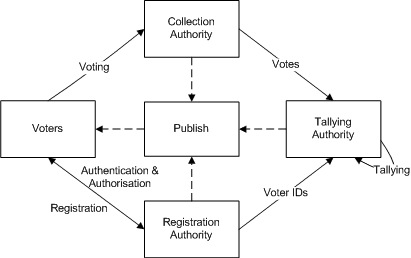
\includegraphics[scale=0.7]{Voting_Process.png}
\centering
\end{figure}


\section{Challenges}


In their paper Damgård, Groth and Gorm outline three important challenges
that need to be solved [DGS02]:

\begin{description}
    \item[Privacy] Only the final result should be made public, no information
        about the votes must be leaked.

    \item[Robustness] The result will reflect all submitted and well-formed ballots
        correctly, even if some voters or entities running the election cheat.

    \item[Universal verifiability] After the election, the result can be verified by
        anyone. In order words, any party should be able to convince himself
        that the election was fair in the sense that the published tally was
        correctly computed.
\end{description}


\section{Security Requirements}

\cite{Cet08}
\begin{itemize}
    \item \textit{Voter Privacy}
        No one should be able to link a vote back to the specific voter, and only the voter should
        know his vote. These requirements shall hold during and after the election.  
    
    \item \textit{Eligibility}    
        Only Eligible and registered voters can vote. 
    
    \item \textit{Uniqueness}
        Only one vote per registered voter should be counted.
    
    \item \textit{Fairness}
        None should be able to gain any knowledge of the outcome of the election, before the ending. This is to prevent voters of voting accordingly to any leaked information. 
    
    \item \textit{Uncoercibility}
        Nobody should be able to extract the value of a vote. This is to prevent anybody from compelling a voter by force, intimidation, or authority to cast a vote in a specific way. 
    
    \item \textit{Receipt-freeness} 
        The voting system should not produce a receipt that reveals any information about the casted vote. This is to prevent a vote from trading his vote. 
    
    \item \textit{Accuracy} 
        The final tally should be correctly computed from valid casted votes. It should not be
        possible to manipulate the final tally without being detected. 
    
    \item \textit{Universal Verifiability}
        It should be possible for any participants and observers to validate individual votes as well as the final tally of the election. 
    
    \item \textit{Individual Verifiability}    
        Every registered voter should be able to verify that his vote is counted correctly. 
    
\end{itemize}

\section{Approaches}

\begin{description}
    \item[Mix-nets] In mix-net voting schemes, the ballots of all voters are shuffled through a
        mix-net, such that afterwards, it is unclear which ballot belongs to which
        voter. More precisely, the voter encrypts his vote consecutively with the
        public key of each mixer, then all these multi-encrypted votes are sequentially
        decrypted and permuted by each mixer. The output of the
        last mixer is a shuffle of the votes in clear, but in random order. These
        votes can then be tallied publicly. In order to guarantee correctness of the
        tally, every mixer must additional publish a proof that he did not modify
        or substitute votes. This process is illustrated in Figure 1.2.
        For the first mixer, the secrecy of the votes is based on the infeasibility
        of decrypting, and with each mixer, the level of encryption is decreased,
        but the level of anonymity of the voter is increased. The correctness is
        22 Introduction
        based on the soundness of the public proofs. Because at the end all votes
        are known in clear, invalid votes can be discarded easily.
    
    
    \item[Blind signatures] This approach can be seen as an abstraction of mix-net voting            schemes. Here, each voter casts his vote unencrypted, but anonymously. The security
        of this scheme is based on hiding which vote belongs to which voter.
        Additional efforts are needed to ensure that only entitled voters can cast
        a vote: Each voter is to get a blindly signed public key from a registration
        authority, with which he signs his vote and sends it over an anonymous
        channel to the bulletin board. This approach is illustrated in Figure 1.3.
        
        
    \item[Homomorphic encryption] A homomorphic encryption scheme supports addition of               ciphertexts without knowledge of the secret key. With this primitive, one can construct
        very efficient voting protocols: The voter encrypts his vote with a
        homomorphic encryption scheme and posts it to the bulletin board. The
        authorities can tally the encrypted votes and decrypt the sum (see Figure
        1.4). In addition, each voter must prove the validity of the submitted
        vote. In this approach, it is clear which (encrypted) vote belongs to which
        voter, and the secrecy of the votes is based on the infeasibility of decrypting
        votes.
\end{description}
